\documentclass[a4paper,leqno,dvipdfmx,draft]{jsarticle}
\usepackage{syuron2}

%\usepackage{amsmath}
%\usepackage{amsfonts}
%\usepackage{amsthm}

% ------------------------
% usepackage
% ------------------------
%\usepackage{algorithm}
\usepackage{algorithmic}
\usepackage{amscd}
\usepackage{amsfonts}
\usepackage{amsmath}
\usepackage[psamsfonts]{amssymb}
\usepackage{amsthm}
\usepackage{ascmac}
\usepackage{bm}
\usepackage{color}
\usepackage{enumerate}
\usepackage{fancybox}
\usepackage[stable]{footmisc}
\usepackage{graphicx}
\usepackage{listings}
\usepackage{mathrsfs}
\usepackage{mathtools}
\usepackage{otf}
\usepackage{pifont}
\usepackage{proof}
\usepackage{subfigure}
\usepackage{tikz}
\usepackage{verbatim}
\usepackage[all]{xy}

\usetikzlibrary{cd}
\usetikzlibrary{arrows.meta}


% ================================
% パッケージを追加する場合のスペース 
\usepackage[dvipdfmx]{hyperref}
\usepackage{xcolor}
\definecolor{darkgreen}{rgb}{0,0.45,0} 
\definecolor{darkred}{rgb}{0.75,0,0}
\definecolor{darkblue}{rgb}{0,0,0.6} 
\hypersetup{
    colorlinks=true,
    %citecolor=darkgreen,
    %linkcolor=darkred,
    %urlcolor=darkblue,
    citecolor=black,
    linkcolor=black,
    urlcolor=black,
}
\usepackage{pxjahyper}

%\usepackage[mathscr]{euscript} % mathscr のフォントを変更

%\usepackage{mmasym}

%=================================


% --------------------------
% theoremstyle
% --------------------------
\theoremstyle{definition}

% --------------------------
% newtheoem
% --------------------------

% 日本語で定理, 命題, 証明などを番号付きで用いるためのコマンドです. 
% If you want to use theorem environment in Japanece, 
% you can use these code. 
% Attention!
% All theorem enivironment numbers depend on 
% only section numbers.
\newtheorem{Axiom}{公理}[section]
\newtheorem{Definition}[Axiom]{定義}
\newtheorem{Theorem}[Axiom]{定理}
\newtheorem{Proposition}[Axiom]{命題}
\newtheorem{Lemma}[Axiom]{補題}
\newtheorem{Corollary}[Axiom]{系}
\newtheorem{Example}[Axiom]{例}
\newtheorem{Claim}[Axiom]{主張}
\newtheorem{Property}[Axiom]{性質}
\newtheorem{Attention}[Axiom]{注意}
\newtheorem{Question}[Axiom]{問}
\newtheorem{Problem}[Axiom]{問題}
\newtheorem{Consideration}[Axiom]{考察}
\newtheorem{Alert}[Axiom]{警告}
\newtheorem{Fact}[Axiom]{事実}


% 日本語で定理, 命題, 証明などを番号なしで用いるためのコマンドです. 
% If you want to use theorem environment with no number in Japanese, You can use these code.
\newtheorem*{Axiom*}{公理}
\newtheorem*{Definition*}{定義}
\newtheorem*{Theorem*}{定理}
\newtheorem*{Proposition*}{命題}
\newtheorem*{Lemma*}{補題}
\newtheorem*{Example*}{例}
\newtheorem*{Corollary*}{系}
\newtheorem*{Claim*}{主張}
\newtheorem*{Property*}{性質}
\newtheorem*{Attention*}{注意}
\newtheorem*{Question*}{問}
\newtheorem*{Problem*}{問題}
\newtheorem*{Consideration*}{考察}
\newtheorem*{Alert*}{警告}
\newtheorem{Fact*}{事実}


% 英語で定理, 命題, 証明などを番号付きで用いるためのコマンドです. 
%　If you want to use theorem environment in English, You can use these code.
%all theorem enivironment number depend on only section number.
\newtheorem{Axiom+}{Axiom}[section]
\newtheorem{Definition+}[Axiom+]{Definition}
\newtheorem{Theorem+}[Axiom+]{Theorem}
\newtheorem{Proposition+}[Axiom+]{Proposition}
\newtheorem{Lemma+}[Axiom+]{Lemma}
\newtheorem{Example+}[Axiom+]{Example}
\newtheorem{Corollary+}[Axiom+]{Corollary}
\newtheorem{Claim+}[Axiom+]{Claim}
\newtheorem{Property+}[Axiom+]{Property}
\newtheorem{Attention+}[Axiom+]{Attention}
\newtheorem{Question+}[Axiom+]{Question}
\newtheorem{Problem+}[Axiom+]{Problem}
\newtheorem{Consideration+}[Axiom+]{Consideration}
\newtheorem{Alert+}{Alert}
\newtheorem{Fact+}[Axiom+]{Fact}
\newtheorem{Remark+}[Axiom+]{Remark}

% ----------------------------
% commmand
% ----------------------------
% 執筆に便利なコマンド集です. 
% コマンドを追加する場合は下のスペースへ. 

% 集合の記号 (黒板文字)
\newcommand{\NN}{\mathbb{N}}
\newcommand{\ZZ}{\mathbb{Z}}
\newcommand{\QQ}{\mathbb{Q}}
\newcommand{\RR}{\mathbb{R}}
\newcommand{\CC}{\mathbb{C}}
\newcommand{\PP}{\mathbb{P}}
\newcommand{\KK}{\mathbb{K}}


% 集合の記号 (太文字)
\newcommand{\nn}{\mathbf{N}}
\newcommand{\zz}{\mathbf{Z}}
\newcommand{\qq}{\mathbf{Q}}
\newcommand{\rr}{\mathbf{R}}
\newcommand{\cc}{\mathbf{C}}
\newcommand{\pp}{\mathbf{P}}
\newcommand{\kk}{\mathbf{k}}

% 特殊な写像の記号
\newcommand{\ev}{\mathop{\mathrm{ev}}\nolimits} % 値写像
\newcommand{\pr}{\mathop{\mathrm{pr}}\nolimits} % 射影

% スクリプト体にするコマンド
%   例えば　{\mcal C} のように用いる
\newcommand{\mcal}{\mathcal}

% 花文字にするコマンド 
%   例えば　{\h C} のように用いる
\newcommand{\h}{\mathscr}

% ヒルベルト空間などの記号
\newcommand{\F}{\mcal{F}}
\newcommand{\X}{\mcal{X}}
\newcommand{\Y}{\mcal{Y}}
\newcommand{\Hil}{\mcal{H}}
\newcommand{\RKHS}{\Hil_{k}}
\newcommand{\Loss}{\mcal{L}_{D}}
\newcommand{\MLsp}{(\X, \Y, D, \Hil, \Loss)}

% 偏微分作用素の記号
\newcommand{\p}{\partial}

% 角カッコの記号 (内積は下にマクロがあります)
\newcommand{\lan}{\langle}
\newcommand{\ran}{\rangle}



% 圏の記号など
\newcommand{\Set}{{\bf Set}}
\newcommand{\Vect}{{\bf Vect}}
\newcommand{\FDVect}{{\bf FDVect}}
%\newcommand{\Ring}{{\bf Ring}}
\newcommand{\Ab}{{\bf Ab}}
\newcommand{\Mod}{\mathop{\mathrm{Mod}}\nolimits}
\newcommand{\Modf}{\mathop{\mathrm{Mod}^\mathrm{f}}\nolimits}
\newcommand{\CGA}{{\bf CGA}}
\newcommand{\GVect}{{\bf GVect}}
\newcommand{\Lie}{{\bf Lie}}
\newcommand{\dLie}{{\bf Liec}}



% 射の集合など
\newcommand{\Map}{\mathop{\mathrm{Map}}\nolimits} % 写像の集合
\newcommand{\Hom}{\mathop{\mathrm{Hom}}\nolimits} % 射集合
\newcommand{\End}{\mathop{\mathrm{End}}\nolimits} % 自己準同型の集合
\newcommand{\Aut}{\mathop{\mathrm{Aut}}\nolimits} % 自己同型の集合
\newcommand{\Mor}{\mathop{\mathrm{Mor}}\nolimits} % 射集合
\newcommand{\Ker}{\mathop{\mathrm{Ker}}\nolimits} % 核
\newcommand{\Img}{\mathop{\mathrm{Im}}\nolimits} % 像
\newcommand{\Cok}{\mathop{\mathrm{Coker}}\nolimits} % 余核
\newcommand{\Cim}{\mathop{\mathrm{Coim}}\nolimits} % 余像

% その他便利なコマンド
\newcommand{\dip}{\displaystyle} % 本文中で数式モード
\newcommand{\e}{\varepsilon} % イプシロン
\newcommand{\dl}{\delta} % デルタ
\newcommand{\pphi}{\varphi} % ファイ
\newcommand{\ti}{\tilde} % チルダ
\newcommand{\pal}{\parallel} % 平行
\newcommand{\op}{{\rm op}} % 双対を取る記号
\newcommand{\lcm}{\mathop{\mathrm{lcm}}\nolimits} % 最小公倍数の記号
\newcommand{\Probsp}{(\Omega, \F, \P)} 
\newcommand{\argmax}{\mathop{\rm arg~max}\limits}
\newcommand{\argmin}{\mathop{\rm arg~min}\limits}





% ================================
% コマンドを追加する場合のスペース 
%\newcommand{\OO}{\mcal{O}}



\makeatletter
\renewenvironment{proof}[1][\proofname]{\par
  \pushQED{\qed}%
  \normalfont \topsep6\p@\@plus6\p@\relax
  \trivlist
  \item[\hskip\labelsep
%        \itshape
         \bfseries
%    #1\@addpunct{.}]\ignorespaces
    {#1}]\ignorespaces
}{%
  \popQED\endtrivlist\@endpefalse
}
\makeatother

\renewcommand{\proofname}{Proof.}



%\renewcommand\proofname{\bf 証明} % 証明
\numberwithin{equation}{section}
\newcommand{\cTop}{\textsf{Top}}
%\newcommand{\cOpen}{\textsf{Open}}
\newcommand{\Op}{\mathop{\textsf{Op}}\nolimits}
\newcommand{\Ob}{\mathop{\textrm{Ob}}\nolimits}
\newcommand{\id}{\mathop{\mathrm{id}}\nolimits}
\newcommand{\pt}{\mathop{\mathrm{pt}}\nolimits}
\newcommand{\res}{\mathop{\rho}\nolimits}
\newcommand{\A}{\mcal{A}}
\newcommand{\B}{\mcal{B}}
\newcommand{\C}{\mcal{C}}
\newcommand{\D}{\mcal{D}}
\newcommand{\E}{\mcal{E}}
\newcommand{\G}{\mcal{G}}
%\newcommand{\H}{\mcal{H}}
\newcommand{\I}{\mcal{I}}
\newcommand{\J}{\mcal{J}}
\newcommand{\OO}{\mcal{O}}
\newcommand{\Ring}{\mathop{\textsf{Ring}}\nolimits}
\newcommand{\cAb}{\mathop{\textsf{Ab}}\nolimits}
%\newcommand{\Ker}{\mathop{\mathrm{Ker}}\nolimits}
\newcommand{\im}{\mathop{\mathrm{Im}}\nolimits}
\newcommand{\Coker}{\mathop{\mathrm{Coker}}\nolimits}
\newcommand{\Coim}{\mathop{\mathrm{Coim}}\nolimits}
\newcommand{\rank}{\mathop{\mathrm{rank}}\nolimits}
\newcommand{\Ht}{\mathop{\mathrm{Ht}}\nolimits}
\newcommand{\supp}{\mathop{\mathrm{supp}}\nolimits}
\newcommand{\colim}{\mathop{\mathrm{colim}}}
\newcommand{\Tor}{\mathop{\mathrm{Tor}}\nolimits}

\newcommand{\cat}{\mathscr{C}}

%筆記体
\newcommand{\cA}{\mcal{A}}
\newcommand{\cB}{\mcal{B}}
\newcommand{\cC}{\mcal{C}}
\newcommand{\cD}{\mcal{D}}
\newcommand{\cE}{\mcal{E}}
\newcommand{\cF}{\mcal{F}}
\newcommand{\cG}{\mcal{G}}
\newcommand{\cH}{\mcal{H}}
\newcommand{\cI}{\mcal{I}}
\newcommand{\cJ}{\mcal{J}}
\newcommand{\cK}{\mcal{K}}
\newcommand{\cL}{\mcal{L}}
\newcommand{\cM}{\mcal{M}}
\newcommand{\cN}{\mcal{N}}
\newcommand{\cO}{\mcal{O}}
\newcommand{\cP}{\mcal{P}}
\newcommand{\cQ}{\mcal{Q}}
\newcommand{\cR}{\mcal{R}}
\newcommand{\cS}{\mcal{S}}
\newcommand{\cT}{\mcal{T}}
\newcommand{\cU}{\mcal{U}}
\newcommand{\cV}{\mcal{V}}
\newcommand{\cW}{\mcal{W}}
\newcommand{\cX}{\mcal{X}}
\newcommand{\cY}{\mcal{Y}}
\newcommand{\cZ}{\mcal{Z}}


\newcommand{\scA}{\mathscr{A}}
\newcommand{\scB}{\mathscr{B}}
\newcommand{\scC}{\mathscr{C}}
\newcommand{\scD}{\mathscr{D}}
\newcommand{\scE}{\mathscr{E}}
\newcommand{\scF}{\mathscr{F}}
\newcommand{\scN}{\mathscr{N}}
\newcommand{\scO}{\mathscr{O}}
\newcommand{\scV}{\mathscr{V}}
\newcommand{\scU}{\mathscr{U}}


\newcommand{\ibA}{\mathop{\text{\textit{\textbf{A}}}}}
\newcommand{\ibB}{\mathop{\text{\textit{\textbf{B}}}}}
\newcommand{\ibC}{\mathop{\text{\textit{\textbf{C}}}}}
\newcommand{\ibD}{\mathop{\text{\textit{\textbf{D}}}}}
\newcommand{\ibE}{\mathop{\text{\textit{\textbf{E}}}}}
\newcommand{\ibF}{\mathop{\text{\textit{\textbf{F}}}}}
\newcommand{\ibG}{\mathop{\text{\textit{\textbf{G}}}}}
\newcommand{\ibH}{\mathop{\text{\textit{\textbf{H}}}}}
\newcommand{\ibI}{\mathop{\text{\textit{\textbf{I}}}}}
\newcommand{\ibJ}{\mathop{\text{\textit{\textbf{J}}}}}
\newcommand{\ibK}{\mathop{\text{\textit{\textbf{K}}}}}
\newcommand{\ibL}{\mathop{\text{\textit{\textbf{L}}}}}
\newcommand{\ibM}{\mathop{\text{\textit{\textbf{M}}}}}
\newcommand{\ibN}{\mathop{\text{\textit{\textbf{N}}}}}
\newcommand{\ibO}{\mathop{\text{\textit{\textbf{O}}}}}
\newcommand{\ibP}{\mathop{\text{\textit{\textbf{P}}}}}
\newcommand{\ibQ}{\mathop{\text{\textit{\textbf{Q}}}}}
\newcommand{\ibR}{\mathop{\text{\textit{\textbf{R}}}}}
\newcommand{\ibS}{\mathop{\text{\textit{\textbf{S}}}}}
\newcommand{\ibT}{\mathop{\text{\textit{\textbf{T}}}}}
\newcommand{\ibU}{\mathop{\text{\textit{\textbf{U}}}}}
\newcommand{\ibV}{\mathop{\text{\textit{\textbf{V}}}}}
\newcommand{\ibW}{\mathop{\text{\textit{\textbf{W}}}}}
\newcommand{\ibX}{\mathop{\text{\textit{\textbf{X}}}}}
\newcommand{\ibY}{\mathop{\text{\textit{\textbf{Y}}}}}
\newcommand{\ibZ}{\mathop{\text{\textit{\textbf{Z}}}}}

\newcommand{\ibx}{\mathop{\text{\textit{\textbf{x}}}}}

%\newcommand{\Comp}{\mathop{\mathrm{C}}\nolimits}
%\newcommand{\Komp}{\mathop{\mathrm{K}}\nolimits}
%\newcommand{\Domp}{\mathop{\mathsf{D}}\nolimits}%複体のホモトピー圏
%\newcommand{\Comp}{\mathrm{C}}
%\newcommand{\Komp}{\mathrm{K}}
%\newcommand{\Domp}{\mathsf{D}}%複体のホモトピー圏

\newcommand{\Comp}{\mathop{\mathrm{C}}\nolimits}
\newcommand{\Komp}{\mathop{\mathsf{K}}\nolimits}
\newcommand{\Domp}{\mathord{\mathsf{D}}}%\nolimits}
\newcommand{\Kompl}{\mathop{\mathsf{K}^\mathrm{+}}\nolimits}
\newcommand{\Kompu}{\mathop{\mathsf{K}^\mathrm{-}}\nolimits}
\newcommand{\Kompb}{\mathop{\mathsf{K}^\mathrm{b}}\nolimits}
\newcommand{\Dompl}{\mathop{\mathsf{D}^\mathrm{+}}\nolimits}
\newcommand{\Dompu}{\mathop{\mathsf{D}^\mathrm{-}}\nolimits}
\newcommand{\Dompb}{\mathop{\mathsf{D}^\mathrm{b}}\nolimits}
\newcommand{\Dompbf}{\mathop{\mathsf{D}_\mathrm{f}^\mathrm{b}}\nolimits}
\newcommand{\Domplb}{\mathop{\mathsf{D}^\mathrm{lb}}\nolimits}




\newcommand{\CCat}{\Comp(\cat)}
\newcommand{\KCat}{\Komp(\cat)}
\newcommand{\DCat}{\Domp(\cat)}%圏Cの複体のホモトピー圏
\newcommand{\HOM}{\mathop{\mathscr{H}\hspace{-2pt}om}\nolimits}%内部Hom
\newcommand{\RHOM}{\mathop{\mathrm{R}\hspace{-1.5pt}\HOM}\nolimits}

%\newcommand{\muS}{\mathop{\mathrm{SS}}\nolimits}
\newcommand{\muS}[1][]{\mathop{\mathrm{SS}}\nolimits_{#1}}
\newcommand{\RG}{\mathop{\mathrm{R}\hspace{-0pt}\Gamma}\nolimits}
\newcommand{\RHom}{\mathop{\mathrm{R}\hspace{-1.5pt}\Hom}\nolimits}
%\newcommand{\Rder}{\mathrm{R}}
\newcommand{\Rder}[1][]{\mathop{\mathrm{R}^{#1}\hspace{-2pt}}\nolimits}

\newcommand{\simar}{\mathrel{\overset{\sim}{\rightarrow}}}%同型右矢印
\newcommand{\simarr}{\mathrel{\overset{\sim}{\longrightarrow}}}%同型右矢印
\newcommand{\simra}{\mathrel{\overset{\sim}{\leftarrow}}}%同型左矢印
\newcommand{\simrra}{\mathrel{\overset{\sim}{\longleftarrow}}}%同型左矢印

\newcommand{\hocolim}{{\mathrm{hocolim}}}
\newcommand{\indlim}[1][]{\mathop{\varinjlim}\limits_{#1}}
\newcommand{\sindlim}[1][]{\smash{\mathop{\varinjlim}\limits_{#1}}\,}
\newcommand{\Pro}{\mathrm{Pro}}
\newcommand{\Ind}{\mathrm{Ind}}
\newcommand{\prolim}[1][]{\mathop{\varprojlim}\limits_{#1}}
\newcommand{\sprolim}[1][]{\smash{\mathop{\varprojlim}\limits_{#1}}\,}

\newcommand{\Sh}{\mathrm{Sh}}
\newcommand{\PSh}{\mathrm{PSh}}

\newcommand{\rmD}{\mathrm{D}}

\newcommand{\Lloc}[1][]{\mathord{\mathcal{L}^1_{\mathrm{loc},{#1}}}}
\newcommand{\ori}{\mathord{\mathrm{or}}}
\newcommand{\Db}{\mathord{\mathscr{D}b}}

\newcommand{\codim}{\mathop{\mathrm{codim}}\nolimits}



\newcommand{\gld}{\mathop{\mathrm{gld}}\nolimits}
\newcommand{\wgld}{\mathop{\mathrm{wgld}}\nolimits}


\newcommand{\tens}[1][]{\mathbin{\otimes_{\raise1.5ex\hbox to-.1em{}{#1}}}}
\newcommand{\etens}{\mathbin{\boxtimes}}
\newcommand{\ltens}[1][]{\mathbin{\overset{\mathrm{L}}\tens}_{#1}}
\newcommand{\mtens}[1][]{\mathbin{\overset{\mathrm{\mu}}\tens}_{#1}}
\newcommand{\lltens}[1][]{{\mathop{\tens}\limits^{\mathrm{L}}_{#1}}}
\newcommand{\letens}{\overset{\mathrm{L}}{\etens}}
\newcommand{\detens}{\underline{\etens}}
\newcommand{\ldetens}{\overset{\mathrm{L}}{\underline{\etens}}}
\newcommand{\dtens}[1][]{{\overset{\mathrm{L}}{\underline{\otimes}}}_{#1}}

\newcommand{\blk}{\mathord{\ \cdot\ }}
\newcommand{\mres}[2][]{{\left.{#1}\right\rvert}_{#2}}


%\newcommand{\hocolim}{{\mathrm{hocolim}}}
%\newcommand{\indlim}[1][]{\mathop{\varinjlim}\limits_{#1}}
%\newcommand{\sindlim}[1][]{\smash{\mathop{\varinjlim}\limits_{#1}}\,}
%\newcommand{\Pro}{\mathrm{Pro}}
%\newcommand{\Ind}{\mathrm{Ind}}
%\newcommand{\prolim}[1][]{\mathop{\varprojlim}\limits_{#1}}
%\newcommand{\sprolim}[1][]{\smash{\mathop{\varprojlim}\limits_{#1}}\,}
\newcommand{\proolim}[1][]{\mathop{\text{\rm``{$\varprojlim$}''}}\limits_{#1}}
\newcommand{\sproolim}[1][]{\smash{\mathop{\rm``{\varprojlim}''}\limits_{#1}}}
\newcommand{\inddlim}[1][]{\mathop{\text{\rm``{$\varinjlim$}''}}\limits_{#1}}
\newcommand{\sinddlim}[1][]{\smash{\mathop{\text{\rm``{$\varinjlim$}''}}\limits_{#1}}\,}
\newcommand{\ooplus}{\mathop{\text{\rm``{$\oplus$}''}}\limits}
\newcommand{\bbigsqcup}{\mathop{``\bigsqcup''}\limits}
\newcommand{\bsqcup}{\mathop{``\sqcup''}\limits}
\newcommand{\dsum}[1][]{\mathbin{\oplus_{#1}}}

\newcommand{\Fct}{\mathop{\mathsf{Fct}}\nolimits}

\newcommand{\pb}[1][]{\mathbin{\mathop{\times}\limits_{#1}}}
\newcommand{\dpb}[1][]{\mathbin{\mathop{\times}\limits_{#1}}}
\newcommand{\tpb}[1][]{\mathbin{\mathop{\times}\nolimits_{#1}}}





%================================================
% 自前の定理環境
%   https://mathlandscape.com/latex-amsthm/
% を参考にした
\newtheoremstyle{mystyle}%   % スタイル名
    {5pt}%                   % 上部スペース
    {5pt}%                   % 下部スペース
    {}%              % 本文フォント
    {}%                  % 1行目のインデント量
    {\bfseries}%                      % 見出しフォント
    {.}%                     % 見出し後の句読点
    {12pt}%                     % 見出し後のスペース
    {\thmname{#1}\thmnumber{ #2}\thmnote{{\hspace{2pt}\normalfont (#3)}}}% % 見出しの書式

\theoremstyle{mystyle}
\newtheorem{AXM}{公理}[section]
\newtheorem{DFN}[AXM]{定義}
\newtheorem{THM}[AXM]{定理}
\newtheorem*{THM*}{定理}
\newtheorem{PRP}[AXM]{命題}
\newtheorem{LMM}[AXM]{補題}
\newtheorem{CRL}[AXM]{系}
\newtheorem{EG}[AXM]{例}
\newtheorem*{EG*}{例}
\newtheorem{RMK}[AXM]{注意}
\newtheorem{CNV}[AXM]{約束}
\newtheorem{CMT}[AXM]{コメント}
\newtheorem*{CMT*}{コメント}
\newtheorem{NTN}[AXM]{記号}

% 定理環境ここまで
%====================================================

\usepackage{framed}
\definecolor{lightgray}{rgb}{0.75,0.75,0.75}
\renewenvironment{leftbar}{%
  \def\FrameCommand{\textcolor{lightgray}{\vrule width 4pt} \hspace{10pt}}% 
  \MakeFramed {\advance\hsize-\width \FrameRestore}}%
{\endMakeFramed}
\newenvironment{redleftbar}{%
  \def\FrameCommand{\textcolor{lightgray}{\vrule width 1pt} \hspace{10pt}}% 
  \MakeFramed {\advance\hsize-\width \FrameRestore}}%
 {\endMakeFramed}



\renewcommand{\Re}{\mathop{\mathrm{Re}}\nolimits}

% =================================





% ---------------------------
% new definition macro
% ---------------------------
% 便利なマクロ集です

% 内積のマクロ
%   例えば \inner<\pphi | \psi> のように用いる
\def\inner<#1>{\langle #1 \rangle}

% ================================
% マクロを追加する場合のスペース 

%=================================



% 位相空間
\newcommand{\Int}[1][]{\mathop{\mathrm{Int}}\nolimits_{#1}}
\newcommand{\Cl}[1][]{\mathop{\mathrm{Cl}}\nolimits_{#1}}
\newcommand{\Bd}[1][]{\mathop{\mathrm{Bd}}\nolimits_{#1}}
\newcommand{\bd}{\mathord{\partial}}
\newcommand{\Fr}[1][]{\mathop{\mathrm{Fr}}\nolimits_{#1}}


\newcommand{\mtan}[1][]{T\hspace{-1.75pt}{#1}}
\newcommand{\mtp}[1][]{{}^{t\!}{#1}} % transpose of the morphism
%\newcommand{\mpb}[1][]{{}^{t\!}{#1}'} % pull-back of the morphism
\newcommand{\mpb}[1][]{{#1}_{\pi}} % pull-back of the morphism
\newcommand{\mdiff}[1][]{{#1}_{d}} % pull-back of the morphism
\newcommand{\mptan}[1][]{{#1}_{\tau}} % pull-back of the morphism


%\newcommand{\pb}[1][]{\mathbin{\mathop{\times}\limits_{#1}}}

\newcommand{\cotb}[1][]{T^{\ast}{#1}}
\newcommand{\conm}[2][]{T_{#1}^{\hspace{0.7pt}\ast}{#2}}
\newcommand{\norb}[2][]{T_{#1}{#2}}

\newcommand{\cotz}[1][]{T^{\ast}_{#1}{#1}}

\newcommand{\cotn}[1][]{\dot{T}^{\ast}{#1}}


\newcommand{\muhom}{\mu hom}
\newcommand{\muHom}[1][]{\mathrm{Hom}^\mu_{\raise1.5ex\hbox to.1em{}#1}}

\newcommand{\mucat}[2][]{\mathsf{D}^{\mathrm{b}}_{#1}(#2)}
%\newcommand{\mucat}[2][]{\mathsf{D}^{\mathrm{b}}_{#1}(#2)}

\newcommand{\conv}[1][]{\mathbin{\mathop{\circ}\limits_{#1}}}


%\newcommand{\lopen}{\mathopen{]}}
%\newcommand{\lclosed}{\mathopen{[}}
%\newcommand{\ropen}{\mathclose{[}}
%\newcommand{\rclosed}{\mathopen{]}}
\newcommand{\lopen}{\mathopen{(}}
\newcommand{\lclosed}{\mathopen{[}}
\newcommand{\ropen}{\mathclose{)}}
\newcommand{\rclosed}{\mathopen{]}}

\newcommand{\sm}{\raisebox{2.33pt}{~\rule{6.4pt}{1.3pt}~}}
%\newcommand{\smi}{\mathbin{\raisebox{2.33pt}{\rule{6.4pt}{1.3pt}}}}
\newcommand{\smi}{-}

\newcommand{\smid}{\mathrel{;}}

%\figre名を英語にする
\renewcommand{\figurename}{Fig.}
%\参考文献名を英語にする
\renewcommand{\refname}{References}



%\theoremstyle{definition}
\newtheorem{defn}{定義}
\newtheorem{thm}[defn]{定理}
\newtheorem{prop}[defn]{命題}
\newtheorem{lemma}[defn]{補題}
\newtheorem{rem}[defn]{注意}

%\documentclass[a4paper]{jarticle}
% として jarticle を使う場合は，上の \usepackage の部分を
%\usepackage[jslayout]{syuron2}
% のように [jslayout] を追加する．

% 以下は修論のフォーマットを参照して記入する．
\title{
  Microlocal Morse Theory and Truncated Microsupport\\
  （超局所モース理論と打切り超局所台）
}
\author{Toshihiro Oshiba}
\date{
  %\today
  2026.3
} % 例. 2024年3月卒業の場合は「2024.3」を記入する．

\begin{document}

%表紙の作成
\maketitle
%=======================================================================================================
% 添削用ヘッダ（提出時に消す）
% 一番上のdraft も消すこと
% 添削時に色をつけた場合はそれも消すこと
\pagestyle{myheadings}
\markright{\today\quad\texttt{\jobname.tex}}
%============================================================================
%目次の作成
\tableofcontents
\section{Introduction}\label{sec:intro}

%In this paper, 
%\textcolor{black}{w}e study microlocal Morse theory. 
%\textcolor{black}{This} is presented, 
%for instance, in \cite{GKS12}. 
%\subsection{\textcolor{black}{Microlocal Sheaf Theory}}

\textcolor{black}{Microlocal Morse theory is a machinary 
to study the propagations of a cohomology 
of complexes of sheaves. 
More generally, this theory is considered as 
a part of microlocal sheaf theory, 
due to Kashiwara and Schapira. 
They defined the notion of 
microsupport of a complex of sheaves around 1980's.} 

\textcolor{black}{To explain more precisely, 
\textcolor{darkgreen}{let us} fix some notations. 
We consider a commutative unital ring \(\kk\) 
of finite global dimension (e.g.,\(\zz\) or a field). 
Let \(X\) be a topological space. 
We denote by \(\Dompb(\kk_X)\) (resp.\ \(\Dompl(\kk_{X})\)) 
the bounded derived category (resp.\ bounded 
from below derived category) of 
sheaves of \(\kk\)-modules on \(X\).} 

\textcolor{black}{If \(M\) is a real manifold of class \(C^{\infty}\) 
and \(F\) a complex of sheaves, 
then the microsupport \(\muS[](F)\) of \(F\) is 
a closed conic (i.e.,stable 
under \(\rr^{+}\)-action) involutive (i.e.,coisotropic) subset 
of the cotangent bundle of \(M\). 
The precise definition is given in Section \ref{sec:t-ss}, 
but roughly speaking, \(\muS[](F)\) describes the (co)directions 
of \(X\) in which the cohomology of \(F\) cannot be extended. 
This notion can be interepreted by analogy with Morse theory. 
Let \(\varphi\) be a real-valued function of class \(C^1\). 
Then we can replace 
the notion of critical points of \(\varphi\) with 
\textcolor{darkgreen}{the} one with respect to \(F\). 
That is to say, we can define a critical point 
with respect to \(F\) by the point \(p\) 
such that \(d\varphi(p)\) belongs to \(\muS[](F)\). 
We can then obtain \textcolor{darkgreen}{an} analogous result 
of Morse theory in a
framework of sheaf theory. 
\textcolor{black}{In Section \ref{sec:t-morse}, we prove a truncated version 
of (a particular case of) 
the microlocal Morse lemma (cf.\ \cite[Proposition 1.8]{GKS12} 
or \cite[Corollary 5.4.19]{KS90}). 
Roughly speaking, this asserts that 
if there is no critical point wtih respect 
to a complex of sheaves, 
we have the natural isomorphism of the cohomologies 
of the sublevel sets of the manifold.}}

%\subsection{\textcolor{black}{Truncated Microsupport}}

%However, we replace the notion of microsupports with
\textcolor{black}{In 2003, 
Kashiwara, Monteiro-Fernandes, and Schapira
introduced the notion of truncated microsupprt in \cite{KFS03a}}, 
in course of the study of solutions of 
boundary value problems of \(\mcal{D}\)-modules. 
\textcolor{black}{The difference between 
microsupports and truncated microsupports 
is as follows. 
\textcolor{black}{On the one hand, 
a point \(p\) in the cotangent bundle \(\cotb[M]\) does 
not belong to the microsupport if and only if 
a certain kind of cohomologies of 
all the degrees vanish. 
On the other hand, the point \(p\) does 
not belong to the truncated microsupport if and only if 
the same kind of cohomologies of all the degrees less than 
a fixed number vanish.}
}
\textcolor{black}
{After they introduced truncated microsupports, 
few properties of truncated microsupports were shown. 
For example, instead of involutivity, 
a microsupport has a property called weak involutivity. 
This is shown also 
by Kashiwara, Monteiro-Fernandes, 
and Schapira in \cite{KFS03b}. 
Some functorial properties of truncated microsupport are 
studited by several authors. See \cite{KFS03a,FM07}. 
These authors studited truncated microsupports
mainly in the context of analytic problems.}

%\subsection{\textcolor{black}{Results}}

\textcolor{black}
{In this paper, 
in contrast to the previous research, 
we shall apply the truncated microsupport 
to \textcolor{darkgreen}{the} study some geometrical problems. 
First we shall} prove a truncated version (Theorem \ref{prp:t-nonchar})
of the noncharacteristic deformation lemma (Proposition \ref{prp:nonchar}). 
\textcolor{black}
{Consider a family of open sets of a Hausdorff space, and a 
complex of sheaves on that space. 
Roughly speaking, 
original version of this theorem asserts that 
if the family is ``noncharacteristic'', in a sence, 
with respect to the complex of sheaves, 
then we can obtain the natural isomorphism 
beteween the derived functors of the functors of 
the global section over the union of the family and 
the derived functors of the functors of the global section over 
a member of the family.}

%\textcolor{black}{
This lemma is one of the most fundamental result 
in microlocal sheaf theory 
used all along \cite{KS90}. 
Thus a truncated version of this lemma 
is also the key result in this paper. 
However, one should notice that 
the original proof of the lemma cannot be applied 
to our truncated version. 
To prove \textcolor{darkgreen}{the} result, 
we \textcolor{darkgreen}{make three modifications 
to the lemma. 
The first one is that we add an assumption to a total space. 
We assume that the space is not only Hausdorff, but also 
satisfies the condition that its open subspaces are paracompact.} 
\textcolor{darkgreen}{The second one is that we weaken the hypothesis of vanishing of 
cohomologies. In the original lemma, we assume that 
the cohomologies of all degrees vanish. However, in our version, 
we assume that the cohomologies of not all degrees 
but degrees less than a certain number vanish. } 
\textcolor{darkgreen}{The third one is that we make an additional assumption of 
the family of deformation. 
}
Therefore, to make this assumption acceptable to the reader, 
we give several examples of families of deformation with figures. 
Then, in turn, we formulate 
\textcolor{black}{truncated version (Theorem \ref{thm:t-morse}) of} 
microlocal morse lemma (Proposition \ref{prp:mu-morse}), 
under the light of truncated microsupport. 
Note that by using the truncated microsupport, we can gain the 
information of the unique continuation. 
More precisely, if \(k\) is an integer and 
we consider the truncated microsupport \(\muS[k](F)\) of 
a bounded complex of sheaves \(F\), 
we can investigate whether 
the cohomology sheaves \(H^{j}(F)\) propagate or not for \(j<k\), 
and in particular, 
whether the continuation \(H^{k}(F)\) is unique or not, 
if it can be extended. 

%In \cite{KFS03a}, they do not study the functorial property of 
%truncated microsupport of direct images of non proper morphisms. 
%We prove this functorial property under non proper direct images. 

%\subsection{Organization}
%\subsection{\textcolor{black}{Organization}}

This paper is organized as follows. 
In Section \ref{sec:review}, 
we review the notations and results from \cite{KS90}. 
In Section \textcolor{black}{\ref{sec:t-ss}}, 
we define truncated microsupport of sheaves, 
due to \cite{KFS03a}. 
In Section \ref{sec:t-nonchar}, 
we prove a truncated version of 
the noncharacteristic deformation lemma. 
Finally in Section \ref{sec:t-morse}, 
we apply the result in Section \ref{sec:t-nonchar} 
to the microlocal Morse theory. 
In Section \ref{sec:t-nonchar}, 
we prove Lemma \ref{clm:ind-nonchar}, which is too long to 
write in the proof of Theorem \ref{prp:t-nonchar}. 

\section{Background Material}\label{sec:review}

In this section, 
we recall some definitions and results \textcolor{black}{of 
homological algebra and sheaf theory including 
the theory of derived categories} from \cite{KS90}, 
following its notations with slight modifications. 

Let \(X\) be a topological space, 
and \(Z\) a locally closed set of \(X\). 
Let us denot by \(i\colon Z\hookrightarrow X\) \textcolor{black}{the} inclusion. 
We use the following functors: 
\[
  \RG_{Z}(\blk) \coloneqq \Rder[]{i_{\ast}}i^{!}, 
  \quad
  (\blk)_{Z}\coloneqq \Rder[]{i_{!}}i^{-1}.
\]
If there is no risk of confusion, 
we will write \(\kk_Z\) rather than \(\kk_{X,Z}\).

\subsection{Geometrical Notions}
Let \(M\) be a real manifold of class \(C^\infty\). 
We denote by \(\pi_{M}\colon \cotb[M] \to M\) 
the cotangent bundle of \(M\). 
If there is no risk of confusion, 
we will write \(\pi\) rather than \(\pi_{M}\). 
If \(f\colon M\to N\) is a morphism of manifolds \textcolor{black}{(i.e.,a \(C^{\infty}\)-map)}, 
then we have the natural diagram\textcolor{darkred}{s}. 
\[\vcenter{\xymatrix{
  TM
    \ar[r]^-{f'}
    \ar[rd]_-{\tau_M} 
  &
  M\dpb[N]TN
    \ar[r]^-{\mptan[f]}
    \ar[d]
    \ar@{}[dr]|\square
  & 
  TN
    \ar[d]^-{\tau_N}
  &
  \cotb[M]
    \ar[rd]_-{\pi_M}
  &
  M\dpb[N]\cotb[N]
    \ar[l]_-{\mdiff[f]}
    \ar[r]^-{\mpb[f]}
    \ar[d]
    \ar@{}[dr]|\square
  &
  \cotb[N]
    \ar[d]^{\pi_N}
  \\
  &
  M
    \ar[r]_-{f}
  &
  N,
  &
  &
  M
    \ar[r]_-{f}
  &
  N.
}}\]
In \textcolor{darkred}{these diagrams}, 
\(\mptan[f]\) and \(\mpb[f]\) denote 
the natural projections\textcolor{black}{,} \(f'\) is defined by 
\((x;v)\mapsto (x;df_{x}v)\), 
and \(\mdiff[f]\) is induced by the transposition of \(f'\). 

\subsection{Approximation by Inductive Limits}

\begin{Proposition+}[{\cite[Proposition 2.5.1]{KS90}}]\label{prop:ks2.5.1}
  Let \(X\) be a topological space, 
  \(Z\) a subspace, \(F\) a sheaf on \(X\). 
  Consider the canonical morhism:
  \[
    \psi\colon \indlim[U]\Gamma(U;F)
    \to 
    \Gamma(Z;F),
  \]
  where \(U\) ranges through the family of 
  open neighborhoods of \(Z\) in \(X\). 
  \textcolor{black}{Then the following hold.}
  \begin{enumerate}[(i)]
    \item The morphism \(\psi\) is injective. 
    \item Assume that \(X\) is Hausdorff and \(Z\) is compact. 
    Then \(\psi\) is an isomorphism.
    \item Assume that \(X\) is paracompact and \(Z\) is closed. 
    Then \(\psi\) is an isomorphism.
  \end{enumerate}
\end{Proposition+}

\textcolor{black}{Note that a} paracompact space 
is by definition a Hausdorff space. 

\subsection{\textcolor{black}{Complement of Homological Algebra}}\label{ssec:ML}

Consider a projective system of abelian groups \(
  \left(M_n,\rho_{n,p}\right)_n
\) indexed by \(\nn\). 
One says that this system satisfies 
the Mittag-Leffler condition (ML \textcolor{black}{condition} for short) 
if for any \(n\in\nn\), the decreasing sequence \(
  (\rho_{n,p}(M_p))_p
\) of subgroups of \(M_n\) is stationary.

For a projective system of abelian groups \((M_{n})_n\), 
we set \[
  M_{\infty}\coloneqq \prolim[n]M_n.
\]

Consider a projective system of complexes
\begin{equation}
  E_n^{\bullet}\colon 
  \cdots\to M_{n}^{j-1}\to M_{n}^{j}\to M_{n}^{j+1}\to\cdots,
\end{equation}
and \textcolor{black}{its} projective limit
\begin{equation}
  E_{\infty}^{\bullet}\colon 
  \cdots
  \to M_{\infty}^{j-1}
  \to M_{\infty}^{j}
  \to M_{\infty}^{j+1}
  \to\cdots.
\end{equation}
Denote by 
\begin{equation}
  \varPhi_{k}\colon H^{k}(E_{\infty}^{\bullet})\to \prolim[n]H^{k}(E_{n}^{\bullet})
\end{equation}
the natural morphism.

\begin{Proposition+}[{\cite[Proposition 1.12.4]{KS90}}]\label{prop:ks1.12.4}
  Assume that for each \(k\in\zz\), 
  the system \(\left(M_{n}^{\textcolor{darkred}{k}}\right)_{n}\) satisfies 
  the ML condition. 
  Then
  \begin{enumerate}[(a)]
    \item for each \(k\in \zz\), the map \(\varPhi_k\) is surjective,
    \item if moreover, for a given \(i\) the system \(\left(H^{i-1}(E_{n}^{\bullet})\right)_{n}\) satisfies the ML condition, then \(\varPhi_i\) is bijective.
  \end{enumerate} 
\end{Proposition+}

The following is called Kashiwara's lemma.

\begin{Proposition+}[{\cite[Proposition 1.12.6]{KS90}}]\label{prop:ks1.12.6}
  Let \(\left(X_s,\rho_{s,t}\colon X_t\to X_s\right)_{(s,(s\leqq t))}\) be 
  a projective system of sets indexed by \(\rr\). 
  Assume that for each \(s\in\rr\), the canonical maps\[
    \lambda_s\colon X_s\to\prolim[r<s]X_r
  \] and \[
    \mu_s\colon \indlim[t>s]X_t\to X_s
  \] are both injective (resp. surjective). 
  Then all the maps \(\rho_{s_{0},s_{1}}\) \((s_0\leqq s_1)\) are 
  injective (resp. surjective).
\end{Proposition+}

\subsection{\textcolor{black}{ML Procedure for Sheaves}}

\textcolor{darkred}{We use the following 
in the proof of Theorem \ref{prp:t-nonchar}.}

\begin{Proposition+}[{\cite[Proposition 2.7.1]{KS90}}]\label{prop:ks2.7.1}
  Let \(X\) be a topological space and let \(F\in\Dompl(\textcolor{darkred}{\kk}_X)\). 
  Let \(\left(U_n\right)_{n\in\nn}\) be an increasing sequence 
  of open subsets of \(X\), \(\left(Z_n\right)_{n\in\nn}\) 
  a decreasing sequence of closed subsets of \(X\). 
  Set \(U\coloneqq\bigcup_{n}U_{n}\), 
  \(Z\coloneqq\bigcap_{n}Z_{n}\). 
  \textcolor{black}{Then the following hold.}
  \begin{enumerate}[(i)]
    \item \label{item:ks2.7.1.1} For any \(j\), the natural map \(
      \varphi_j\colon H^{j}_{Z}(U;F)
      \to 
      \prolim[n]H^{j}_{Z_{n}}(U_{n};F)
    \) is surjective. 
    \item \label{item:ks2.7.1.2} Assume that for a given \(j\), 
    the projective system \(
      (H^{j-1}_{Z_{n}}(U_{n};F))_{n}
    \) satisfies the ML condition. 
    Then \(\varphi_{j}\) is bijective. 
    \item \label{item:ks2.7.1.3} Let now \(\left(X_{n}\right)_{n\in\nn}\) be 
    an increasing family of subsets of \(X\) satisfying \(
      X=\bigcup_{n}X_n\) and \(X_{n}\subset \Int[](X_{n+1})
    \) for all \(n\). 
    Assume that for a given \(j\), the projective system \(
      \left(H^{j-1}(X_{n};F)\right)_{n}
    \) satisfies the ML condition. 
    Then the natural map \(
      H^{j}(X;F)\to \prolim[n]H^{j}(X_{n};F)
    \) is bijective. 
  \end{enumerate}
\end{Proposition+}

\section{Truncated Microsupport}\label{sec:t-ss}

We give in this section 
the definition of a truncated microsupport 
and 
its functorial property under direct images of proper morphisms. 
\textcolor{black}{Before that, 
we review the original definition of a microsupport. 
\begin{Definition+}[{\cite[Definition 5.1.2]{KS90}}]
  Let \(F\in\Dompb(\kk_X)\). 
  The closed conic subset \(\muS[](F)\) of \(\cotb[X]\) 
  is defined by following condition: \(p\notin \muS[](F)\) 
  if and only if 
  there exists an open neighborhood \(U\) of \(p\) 
  such that for any \(x\in \pi(U)\) and 
  for any real-valued \(C^{1}\)-function \(\varphi\) 
  defined on a neighborhood of \(x\) such that 
  \(\varphi(x)=0\), \(d\varphi(x)\in U\), 
  one has \begin{equation}
    \RG_{\{\varphi\geqq0\}}(F)_x=0.
  \end{equation}
\end{Definition+}
}

\textcolor{black}{Kashiwara, Monteiro-Fernandes, 
and Schapira modified
this definition and gave the notion of truncated microsupport.}

\begin{Definition+}
  Let \(F\in\Dompb(\kk_X)\)\textcolor{darkred}{, and fix an 
  integer \(k\in\zz\)}. 
  \textcolor{darkred}{The \emph{truncated microsupport} \(\muS[k](F)\) is} 
  the closed conic subset of \(\cotb[X]\) 
  defined by \textcolor{darkred}{the following condition}: 
  \(p\notin \muS[k](F)\) 
  if and only if 
  there exists an open conic neighborhood \(U\) of \(p\) 
  such that for any \(x\in \pi(U)\) and 
  for any real-valued \(C^{1}\)-function \(\varphi\) 
  defined on a neighborhood of \(x\) such that 
  \(\varphi(x)=0\), \(d\varphi(x)\in U\), 
  one has \begin{equation}
    H^{j}_{\{\varphi\geqq0\}}(F)_x=0
    \quad \text{for any \(j\leqq k\).}
  \end{equation}
\end{Definition+}

\textcolor{black}{For other equivalent conditions of 
the definition, see \cite{KFS03a}. 
Truncated microsupports satisfy 
the following functorial property under proper direct images.}

\begin{Proposition+}
  Let \(f\colon X\to Y\) be a morphism of 
  manifolds and let \(F\in\Dompb(\kk_X)\) such that \(f\) is proper on \(\supp(F)\). 
  Then for any \(k\in\zz\), 
  \begin{equation}\label{eq:t-push}
    \muS[k](\Rder{f_{\ast}}F)\subset
    \mpb[f]\mdiff[f]^{-1}(\muS[k](F)).
  \end{equation}
  The equality holds in case \(f\) is a closed embedding.
\end{Proposition+}

For other functorial properties, see \cite{KFS03a,FM07}. 

\section{Truncated Noncharacteristic Deformation Lemma}\label{sec:t-nonchar}

In this section, we prove a truncated version of 
the noncharacteristic deformation lemma. 
First we state the result. 
After giving several example, 
we prove Theorem \ref{prp:t-nonchar}. 
In course of the proof, 
we use the key lemma (Lemma \ref{clm:ind-nonchar}). 
Since its proof is rather long, 
we postpone the proof until Section \ref{sec:proof-lem}. 

\textcolor{black}{
Before we state the truncated version, let us review the original 
version of the noncharacteristic deformation lemma.   
%This lemma is originally stated as follows.
\begin{Proposition+}[{\cite[Proposition 2.7.2]{KS90}}]\label{prp:nonchar}
  Let \(X\) be a Hausdorff space. 
  Let \(F\in\Dompl(\kk_X)\), and 
  \(\left(U_{t}\right)_{t\in\rr}\) be a family of 
  open subsets of \(X\). 
  We assume the following conditions. 
  \begin{enumerate}[(i)]
    \item \label{item:nonchar1}
    \(U_{t}=\bigcup_{s<t}U_{s}\), for all \(t\in\rr\). 
    \item \label{item:nonchar2}
    For all pairs \((s,t)\) with \(s\leqq t\), 
    the set \(\overline{U_{t}\smi U_{s}}\cap \supp{F}\) is compact.
    \item \label{item:nonchar3}
    Setting \(
      Z_{s}\coloneqq \bigcap_{t>s}\overline{U_t\smi U_s}
    \), we have
    for all pairs \((s,t)\) with \(s\leqq t\) and 
    all \(x\in Z_{s}\smi U_{t}\), 
    \[
      (\RG_{X\smi U_{t}}(F))_{x}=0.
    \]
  \end{enumerate}
  Then, for all \(t\in\rr\), we have the isomorphisms\[
    \RG\left(\bigcup_{s\in\rr}U_{s};F\right)
    \simar 
    \RG\left(U_{t};F\right).
  \]
\end{Proposition+}
}

Our result is as follows. 

\begin{Theorem+}[Truncated Noncharacteristic Deformation Lemma]\label{prp:t-nonchar}
  Let \(X\) be a Hausdorff space 
  \textcolor{darkgreen}{such that 
  all the open subsets are paracompact}. 
  Let \(F\in\Dompl(\kk_X)\), and 
  \(\left(U_{t}\right)_{t\in\rr}\) be a family of 
  open subsets of \(X\). 
  Let \(k\in\zz\). 
  \textcolor{black}{For \(s\in\rr\)}, set \(
    Z_{s}\coloneqq \bigcap_{t>s}\overline{U_t\smi U_s}
  \). 
  We assume the following conditions. 
  \begin{enumerate}[(i)]
    \item \label{item:t-nonchar1}
    \(U_{t}=\bigcup_{s<t}U_{s}\), for all \(t\in\rr\). 
    \item \label{item:t-nonchar2}
    For all pairs \((s,t)\) with \(s\leqq t\), 
    the set \(\overline{U_{t}\smi U_{s}}\cap \supp{F}\) is compact.
    \item \label{item:t-nonchar3}
    For all \(s\in\rr\) and all \(x\in Z_{s}\smi U_{s}\), 
    we have\[
      (H^{j}_{X\smi U_{s}}(F))_{x}=0
      \quad 
      \text{for all \(j\leqq k\).}
    \]
    \item \label{item:t-nonchar4} 
    For all pairs \((s,t)\) with \(s< t\), \textcolor{darkred}{we have} \(Z_s\subset U_{t}\).
  \end{enumerate}
  Then, for all \(t\in\rr\), we have the isomorphisms\[
    H^{j}\left(\bigcup_{s\in\rr}U_{s};F\right)
    \simar 
    H^{j}\left(U_{t};F\right)
    \quad \text{for all \(j< k\),} 
  \]
  and the \textcolor{darkred}{monomorphisms} \[
    H^{k}\left(\bigcup_{s\in\rr}U_{s};F\right)
    \hookrightarrow 
    H^{k}\left(U_{t};F\right).
  \] 
\end{Theorem+}

\textcolor{black}{Before we prove Theorem \ref{prp:t-nonchar}, 
let us give several examples of families of deformation. 
}
\begin{Example+}\label{eg:t-nonchar}
  The condition \eqref{item:t-nonchar4} of 
  \textcolor{black}{Theorem \ref{prp:t-nonchar}} is not contained 
  in the original version (\textcolor{black}{Proposition \ref{prp:nonchar}}). 
  Therefore let us give an example of \(\left(U_{t}\right)_{t}\) 
  that does not satisfy the condition \eqref{item:t-nonchar4}. 
  \begin{enumerate}[(i)]
    \item \label{item:not-gentle} 
    Let \(X=\rr^2\), and for a real number \(t\) define the 
    function\[
      \varphi_{t}(x)\coloneqq\begin{cases}
        \max\left(0,t(2-\left|x\right|)\right)&(\left|x\right| < 2),\\
        0& (\left|x\right|\geqq 2).
      \end{cases}
    \]
    Then let us denote by \(U_{t}\) the open subset of \(X\)
    \[
      U_{t}\coloneqq
      \left\{
        (x,y)\in X;\ y<\varphi_{t}(x)
      \right\}. 
    \]
    This family \((U_{t})_{t}\) does not satisfy 
    the condition \eqref{item:t-nonchar4}. 
    Indeed, if \(\textcolor{darkred}{0<s<t}\), 
    we have 
    \[
      Z_{s}=\left\{
        (x,y)\in X;\ y=\varphi_{s}(x)\textcolor{darkred}{, \left|x\right|<2}
      \right\}
    \] and the point \((2,0)\in Z_{s}\) is 
    not contained in \(U_{t}\). 
    Moreover, let us \textcolor{black}{define 
    a locally closed subset \(Z\) of \(X\) by}
    \[
      Z\coloneqq \left\{(x,y)\in X;\ (x+2)^{2}+(y-1)^{2}=1\right\}\setminus \left\{(-1,0)\right\}. 
    \]
    For this \(Z\) 
    we denote by \(\kk_{Z}\) the sheaf on \(X\) as \textcolor{darkred}{in} Section \ref{sec:review}. 
    If \(j\leqq0\), we have \(
      H^{j}_{X\smallsetminus U_{t}}(\kk_{Z})_{x}=0
    \) for all \(\textcolor{darkred}{t \geqq s}\) and \(x\in Z_{s}\smallsetminus U_{t}\), 
    but the morhism \(
      H^{0}(U_{1};\kk_{Z})=\kk
      \to 
      0 = H^{0}(U_{0};\kk_{Z})
    \) is not injective. 
    This give an example that 
    satisfies the conditions 
    \eqref{item:t-nonchar1}--\eqref{item:t-nonchar3} but 
    not \eqref{item:t-nonchar4}, 
    which result\textcolor{black}{s} in that 
    the consequence of the proposition does not hold. 
    Hence the condition \eqref{item:t-nonchar4} is necessary. 
    \begin{figure}[htb]
      \centering
      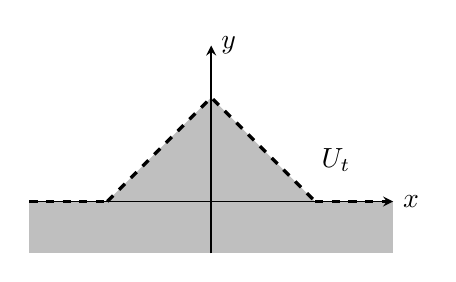
\begin{tikzpicture}[scale=0.66]
        \def\t{1}
        \def\xmax{3.5}
        \def\ymin{-1}
        \def\ymax{3}

        %------------------
        % 塗りつぶし
        %------------------

        % y<0 の部分
        \fill[black!25] (-\xmax,0) rectangle (\xmax,\ymin);

        % 三角形部分 y < t(2-|x|)
        \fill[black!25]
          (-2,0) -- (0,{2*\t}) -- (2,0) -- cycle;

        %------------------
        % 境界（点線）
        %------------------

        % 折れ線
        \draw[very thick,dashed] (-2,0)--(0,{2*\t})--(2,0);

        % x軸（|x|>=2）
        \draw[very thick,dashed] (-\xmax,0)--(-2,0);
        \draw[very thick,dashed] (2,0)--(\xmax,0);

        %------------------
        % 軸
        %------------------

        \draw[->,>=stealth,semithick] (-\xmax,0)--(\xmax,0) node[right]{\(x\)};
        \draw[->,>=stealth,semithick] (0,\ymin)--(0,\ymax) node[right]{\(y\)};

        % ラベル
        \node at (2.4,0.8) {\(U_t\)};
      \end{tikzpicture}
      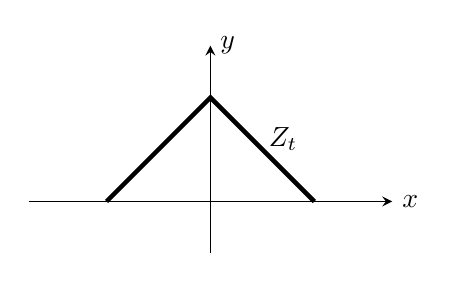
\begin{tikzpicture}[scale=0.66]
        \def\t{1}
        \def\xmax{3.5}
        \def\ymin{-1}
        \def\ymax{3}

        %------------------
        % 境界（点線）
        %------------------

        % 折れ線
        \draw[ultra thick] (-2,0)--(0,{2*\t})--(2,0);
        %------------------
        % 軸
        %------------------

        \draw[->,>=stealth,semithick] (-\xmax,0)--(\xmax,0) node[right]{\(x\)};
        \draw[->,>=stealth,semithick] (0,\ymin)--(0,\ymax) node[right]{\(y\)};

        % ラベル
        \node at (1.4,1.2) {\(Z_t\)};
      \end{tikzpicture}
      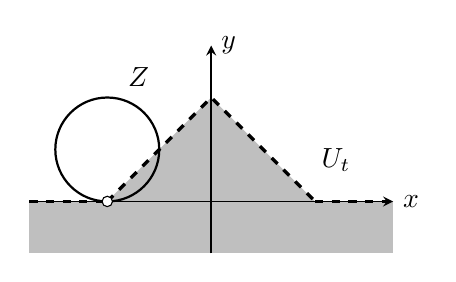
\begin{tikzpicture}[scale=0.66]
        \def\t{1}
        \def\xmax{3.5}
        \def\ymin{-1}
        \def\ymax{3}

        %------------------
        % 塗りつぶし
        %------------------

        % y<0 の部分
        \fill[black!25] (-\xmax,0) rectangle (\xmax,\ymin);

        % 三角形部分 y < t(2-|x|)
        \fill[black!25]
          (-2,0) -- (0,{2*\t}) -- (2,0) -- cycle;

        %------------------
        % 境界（点線）
        %------------------

        % 折れ線
        \draw[very thick,dashed] (-2,0)--(0,{2*\t})--(2,0);

        % x軸（|x|>=2）
        \draw[very thick,dashed] (-\xmax,0)--(-2,0);
        \draw[very thick,dashed] (2,0)--(\xmax,0);

        %------------------
        % 軸
        %------------------

        \draw[->,>=stealth,semithick] (-\xmax,0)--(\xmax,0) node[right]{\(x\)};
        \draw[->,>=stealth,semithick] (0,\ymin)--(0,\ymax) node[right]{\(y\)};

        % 円
        \def\s{1} % 半径 t > 0
        \draw[thick] (-2,1) circle (\s);
        \fill[black!0](-2,0) circle (0.1);
        \draw (-2,0) circle (0.1);

        % ラベル
        \node at (2.4,0.8) {\(U_t\)};
        \node at (-1.4,2.4) {\(Z\)};
      \end{tikzpicture}
      \caption{example \eqref{item:not-gentle}}
      \label{fig:not-gentle}
    \end{figure}
  \end{enumerate}
  Let us, in turn, give three examples 
  of \(\left(U_{t}\right)_{t}\) 
  satisfying the condition \eqref{item:t-nonchar4}. 
  In all the examples below, \(X\) is \(\rr^{2}\). 
  \begin{enumerate}[(i)]
    \setcounter{enumi}{1}
    \item \label{item:gentle1}
    For a real number \(t\), 
    define the open set \(U_{t}\) \textcolor{black}{of \(X\)} 
    by \[
      U_{t}\coloneqq
      \begin{cases}
      \left\{(x,y)\in X;\ \textcolor{darkred}{x^{2}+y^{2}} <t\right\}&(t>0),\\
      \varnothing&(t\leqq0).         
      \end{cases}
    \]
    \begin{figure}[htb]
      \centering
      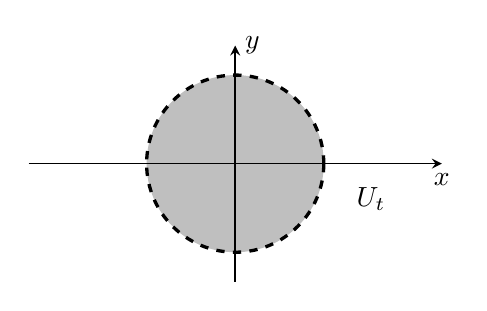
\begin{tikzpicture}[scale=0.75]
        \def\t{1.5} % 半径 t > 0

        % 塗りつぶし
        \fill[black!25] (0,0) circle (\t);

        % 境界
        \draw[dashed, very thick] (0,0) circle (\t);

        % 軸
        \draw[->,>=stealth,semithick] (-3.5,0)--(3.5,0) node[below]{\(x\)};
        \draw[->,>=stealth,semithick] (0,-2)--(0,2) node[right]{\(y\)};
        \node at (2.3,-0.6) {\(U_t\)};
      \end{tikzpicture}
      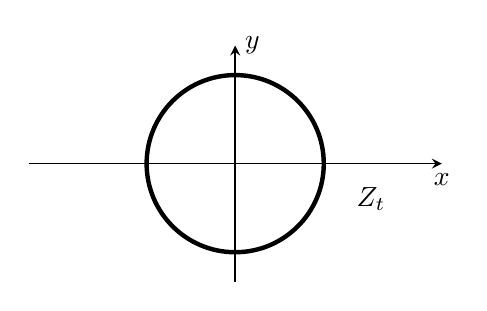
\begin{tikzpicture}[scale=0.75]
        \def\t{1.5} % 半径 t > 0

        % 塗りつぶし
        %\fill[black!25] (0,0) circle (\t);

        % 境界
        \draw[ultra thick] (0,0) circle (\t);

        % 軸
        \draw[->,>=stealth,semithick] (-3.5,0)--(3.5,0) node[below]{\(x\)};
        \draw[->,>=stealth,semithick] (0,-2)--(0,2) node[right]{\(y\)};
        \node at (2.3,-0.6) {\(Z_t\)};
      \end{tikzpicture}
      \caption{example \eqref{item:gentle1}}
      \label{fig:gentle1}
    \end{figure}
    \item \label{item:gentle2}
    For a real number \(t\), 
    define the function \(\varphi_{t}\colon \rr\to \rr\) as follows.
    If \(t\leqq 0\), set \(\varphi_{t}(x)\equiv 0\). 
    If \(t> 0\), set \[
      \varphi_{t}(x)\coloneqq\begin{cases}
        \sqrt{t^{2}-x^{2}} & (\left|x\right|<\textcolor{darkred}{t}),\\
        0&(\left|x\right|\geqq \textcolor{darkred}{t}).
      \end{cases}
    \]
    Then define the open set \(U_{t}\) 
    \textcolor{black}{of \(X\)} by \[
      U_{t}\coloneqq
      \left\{(x,y)\in X;\ y<\varphi_{t}(x)\right\}. 
    \]
    \begin{figure}[htb]
      \centering
      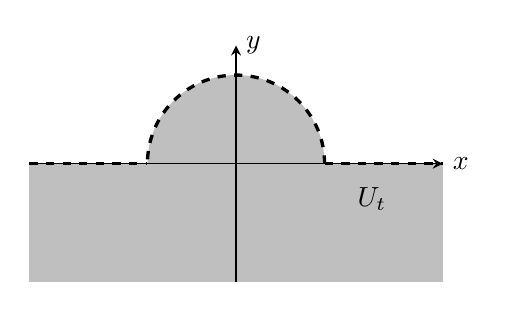
\begin{tikzpicture}[scale=0.75]
        \def\t{1.5}

        %------------------
        % 塗りつぶし領域
        %------------------

        % 半円の下側 y < sqrt(t^2 - x^2)
        \fill[black!25,domain=-\t:\t,samples=200]
          (-\t,0)
          -- plot(\x,{sqrt(\t*\t-\x*\x)})
          -- (\t,0)
          -- cycle;
        \draw[dashed, very thick](0,0) ellipse (1.5 and 1.5);

        % y < 0 の部分
        \fill[black!25] (-3.5,0) rectangle (3.5,-2);

        %------------------
        % 境界
        %------------------

        % 半円（上半分）
        %\draw[thick,domain=-\t:\t,samples=300]
        %  plot(\x,{sqrt(\t*\t-\x*\x)});

        % x軸（|x|>=t の境界として）
        \draw[dashed, very thick] (-3.5,0)--(-\t,0);
        \draw[dashed, very thick] (\t,0)--(3.5,0);

        %------------------
        % 軸
        %------------------

        \draw[->,>=stealth,semithick] (-3.5,0)--(3.5,0) node[right]{\(x\)};
        \draw[->,>=stealth,semithick] (0,-2)--(0,2) node[right]{\(y\)};

        % ラベル
        \node at (2.3,-0.6) {\(U_t\)};
      \end{tikzpicture}
      \begin{tikzpicture}[scale=0.75]
        \def\t{1.5}

        %------------------
        % 塗りつぶし領域
        %------------------

        % 半円の下側 y < sqrt(t^2 - x^2)
        \fill[black!0,domain=-\t:\t,samples=200]
          (-\t,0)
          -- plot(\x,{sqrt(\t*\t-\x*\x)})
          -- (\t,0)
          -- cycle;
        \draw[ultra thick](0,0) ellipse (1.5 and 1.5);

        % y < 0 の部分
        \fill[black!0] (-3.5,0) rectangle (3.5,-2);

        %------------------
        % 境界
        %------------------

        % 半円（上半分）
        %\draw[thick,domain=-\t:\t,samples=300]
        %  plot(\x,{sqrt(\t*\t-\x*\x)});

        % x軸（|x|>=t の境界として）
        %\draw[dashed, very thick] (-3.5,0)--(-\t,0);
        %\draw[dashed, very thick] (\t,0)--(3.5,0);

        %------------------
        % 軸
        %------------------

        \draw[->,>=stealth,semithick] (-3.5,0)--(3.5,0) node[right]{\(x\)};
        \draw[->,>=stealth,semithick] (0,-2)--(0,2) node[right]{\(y\)};

        % ラベル
        \node at (2.1,0.6) {\(Z_t\)};
      \end{tikzpicture}
      \caption{example \eqref{item:gentle2}}
      \label{fig:gentle2}
    \end{figure}
    \item \label{item:gentle3}
    For a real number \(t\), 
    define the open set \(U_{t}\) \textcolor{black}{of \(X\)} 
    as follows. 
    If \(t\leqq0\), set \[
      U_{t}\coloneqq
      \left\{(x,y)\in X;\ y<0\right\}. 
    \]
    If \(t>0\), set \[
      U_{t}\coloneqq
      \left\{(x,y)\in X;\ 
        \begin{array}{cc}
          \text{If \(\left|x\right|<\tfrac{1}{t}\),}&y<t.\vspace{2pt}\\
          \text{Otherwise,}&y<\tfrac{1}{\left|x\right|}.
        \end{array}
      \right\}. 
    \]
    \begin{figure}[htb]
      \centering
      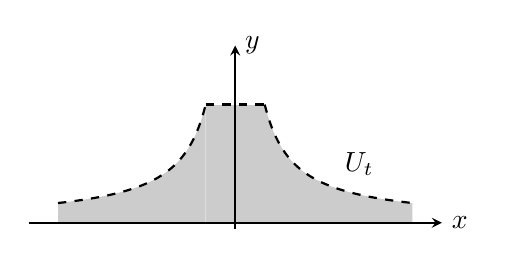
\begin{tikzpicture}[scale=0.75]
        \def\t{2}
        \def\a{1/\t}
        % --- 塗りつぶし部分 ---

        % 中央部分 |x|<1/t, y<t
        \fill[black!20]
          (-\a,0) rectangle (\a,\t);

        % 右側 |x|>=1/t
        \fill[black!20,domain=\a:3,samples=200]
          (\a,0)
          -- plot(\x,{1/\x})
          -- (3,0)
          -- cycle;

        % 左側 |x|>=1/t
        \fill[black!20,domain=-3:-\a,samples=200]
          (-3,0)
          -- plot(\x,{1/abs(\x)})
          -- (-\a,0)
          -- cycle;

        % --- 境界線 ---

        % 水平線 y=t
        \draw[dashed, thick] (-\a,\t)--(\a,\t);

        % 双曲線
        \draw[dashed, thick,domain=\a:3,samples=200]
          plot(\x,{1/\x});
        \draw[dashed, thick,domain=-3:-\a,samples=200]
          plot(\x,{1/abs(\x)});

        % 軸
        \draw[->,>=stealth,semithick] (-3.5,0)--(3.5,0) node[right]{\(x\)};
        \draw[->,>=stealth,semithick] (0,-0.1)--(0,3) node[right]{\(y\)};

        % 補助線
        %\draw[dashed] (\a,0)--(\a,2);
        %\draw[dashed] (-\a,0)--(-\a,2);

        % ラベル
        \node at (2.1,1) {\(U_t\)};
      \end{tikzpicture}
      \begin{tikzpicture}[scale=0.75]
        \def\t{2}
        \def\a{1/\t}

        % 軸
        \draw[->,>=stealth,semithick] (-3.5,0)--(3.5,0) node[right]{\(x\)};
        \draw[->,>=stealth,semithick] (0,-0.1)--(0,3) node[right]{\(y\)};

        % --- 塗りつぶし部分 ---

        % --- 境界線 ---

        % 水平線 y=t
        \draw[ultra thick] (-\a,\t)--(\a,\t);
        % ラベル
        \node at (1.2,2) {\(Z_t\)};
      \end{tikzpicture}
      \caption{example \eqref{item:gentle3}}
      \label{fig:gentle3}
    \end{figure}
  \end{enumerate}
  %These families are visualized as in Figure \ref{fig:1}.
\end{Example+}



\begin{proof}[{\textcolor{black}{Proof of Theorem \ref{prp:t-nonchar}}}]
  Consider the following conditions for 
  \(j\in\zz\) and \(s\in\rr\):
  \begin{align}
      \tag*{\((a)^j_s\)}\label{eq:t-nonchar-a}
      \mu_{s}^{j}&\colon
      \indlim[t>s] H^{j}(U_t;F) \simar H^{j}(U_s;F),\\
      \tag*{\((a')^k_s\)}\label{eq:t-nonchar-a'}
      \mu_{s}^{k}&\colon
      \indlim[t>s] H^{k}(U_t;F) \hookrightarrow H^{k}(U_s;F),\\
      \tag*{\((b)^j_s\)}\label{eq:t-nonchar-b}
      \lambda_{s}^{j}&\colon
      H^{j}(U_s;F)\simarr \prolim[r<s] H^{j}(U_r;F).
  \end{align}

  Let us prove, 
  for all \(s\in \rr\), 
  \ref{eq:t-nonchar-a} for \(j<k\) and \ref{eq:t-nonchar-a'}. 
  We may assume that \(\overline{U_{t}\smi U_{s}}\) is compact 
  for any \(s\leqq t\) by replacing \(X\) by \(\supp{F}\). 
  Consider the distinguished triangle\[
    \RG_{X\smi U_{s}}(F)
    \to
    F
    \to
    \RG_{U_{s}}(F)
    \overset{+1}{\longrightarrow}.
  \]
  Let us endow with \(Z_{s}\cup U_{s}\) the induced topology, and
  denote by \(
    i_{s}\colon Z_{s}\cup U_{s}\hookrightarrow X
  \) the natural continuous map.  
  Applying the functor \[
    \mres[(\blk)]{Z_{s}\cup U_{s}}=i_{s}^{-1}
  \] to the distiguished triangle above, we have \[
    \mres[\RG_{X\smi U_{s}}(F)]{Z_{s}\cup U_{s}}  
    \to
    \mres[F]{Z_{s}\cup U_{s}}  
    \to
    \mres[\RG_{U_{s}}(F)]{Z_{s}\cup U_{s}}  
    \overset{+1}{\longrightarrow}.
  \]
  Again applying to this triangle 
  the functor \(\RG(Z_{s}\cup U_{s};\blk)\), 
  we have
  \begin{equation}
    \RG(Z_{s}\cup U_{s};\RG_{X\smi U_{s}}(F))
    \to
    \RG(Z_{s}\cup U_{s};Z_{s}\cup U_{s})
    \to
    \RG(U_{s};F)
    \overset{+1}{\longrightarrow}. 
  \end{equation}
  By the hypothesis \eqref{item:t-nonchar3} and 
  the definition of a local cohomology, 
  we see that
  \[
    \mres[H^{j}_{X\smi U_{s}}(F)]{Z_{s}\cup U_{s}}=0
    \quad
    \text{for any \(j\leqq k\),}
  \]
  and then \[
    H^{j}\left(Z_{s}\cup U_{s};
      \RG_{X\smi U_{s}}(F)
    \right)=0
    \quad
    \text{for any \(j\leqq k\).}
  \]
  Thus we have
  \begin{align}
    \label{eq:a-iso}
    H^{j}(Z_{s}\cup U_{s};F)
    &\simar
    H^{j}(U_{s};F)\quad
    \text{for any \(j< k\),}\\
    \label{eq:a-inj}
    H^{k}(Z_{s}\cup U_{s};F)
    &\hookrightarrow
    H^{k}(U_{s};F).
  \end{align}
  Therefore, if we show Lemma \ref{clm:ind-nonchar} below, 
  \textcolor{darkred}{whose proof will be given in Section \ref{sec:proof-lem},}
  we have 
  \begin{align*}
    \indlim[t>s]H^{j}(U_t;F)
    &\cong 
    H^{j}(Z_{s}\cup U_{s};F)\\
    &\simar
    H^{j}(U_s;F)
  \end{align*}
  for any \(j<k\), and \ref{eq:t-nonchar-a} follows. 
  Similarly, 
  we have
  \begin{align*}
    \indlim[t>s]H^{k}(U_t;F)
    &\cong 
    H^{k}(Z_{s}\cup U_{s};F)\\
    &\hookrightarrow
    H^{k}(U_s;F)
  \end{align*}
  and \ref{eq:t-nonchar-a'} follows. 
  \begin{Lemma+}\label{clm:ind-nonchar}
    For any \(j\in\zz\) and \(s\in\rr\), there exists a natural isomorphism 
    \[
      \indlim[t>s]H^{j}(U_t;F)
      \cong 
      H^{j}(Z_{s}\cup U_{s};F).
    \]
  \end{Lemma+}

  %Let us come back to the proof of 
  %\textcolor{black}{Theorem \ref{prp:t-nonchar}}. 
  We prove \ref{eq:t-nonchar-b} for 
  all \(j\in\zz\) and \(s\in\rr\) by induction on \(j\). 
  Since \(F\in\Dompl(\kk_X)\), 
  we have \ref{eq:t-nonchar-b} for \(j\ll 0\) and \(s\in\rr\). 
  Hence there exists an integer \(j_{0}<k\) 
  such that \((b)_{s}^{j}\) holds 
  for any \(j<j_{0}\) and \(s\in\rr\).  
  Then assume \ref{eq:t-nonchar-b} is proved for 
  all \(j< j_{0}\) and \(s\in\rr\). 
  Since we have \ref{eq:t-nonchar-a} and \ref{eq:t-nonchar-b} 
  for each \(j< j_{0}\) and each \(s\in\rr\), 
  we can apply 
  Kashiwara's lemma (Proposition \ref{prop:ks1.12.6}) 
  and have\[
    H^{j}(U_{t};F)\simar H^{j}(U_{s};F) 
    \quad
    \text{ for \(j< j_{0}\) and \(s\leqq t\). }
  \]
  Fix \(s\in\rr\) and consider the projective system \(
    \left(H^{j_{0}-1}(U_{s-1/n})\right)_{n\in\nn}
  \). This system satisfies ML condition.  
  Therefore, by applying 
  Proposition \ref{prop:ks2.7.1} (\ref{item:ks2.7.1.3}), 
  %\footnote{
  %  \cite{KS90}の証明だと``by Proposition 1.12.4''
  %  としているが，Proposition 2.7.1の誤植かもしれない．
  %  どちらでも良いとは思うが，
  %  このあと``Again by Proposition 2.7.1'' と書いていることからも，
  %  誤植だと思う方が自然と思われる．
  %}, 
  we have \[
    H^{j}(U_{s};F)
    \simar 
    \prolim[n]H^{j}\left(U_{s-\frac{1}{n}};F\right). 
  \]
  Since \((s-1/n)_{n}\) is a cofinal family of \((t)_{s>t}\), 
  we have \((b)_{s}^{j_{0}}\). 
  Then by induction on \(j\), 
  we have \((b)_{s}^{j}\) for \(j<k\) and \(s\in\rr\). 
  Again by applying Proposition \ref{prop:ks2.7.1} to the 
  projective system \(\left(H^{j}(U_{n};F)\right)_{n}\), 
  we obtain 
  \begin{align*}
    H^{j}\left(\bigcup_{s\in\rr}U_{s};F\right)
    &\cong
    H^{j}\left(\bigcup_{n\in\nn}U_{n};F\right)\\
    &\simar 
    \prolim[n]H^{j}\left(U_{n};F\right)
    %\quad \text{for all \(j< k\),} 
  \end{align*}
  and for each \(n\), we have by Kashiwara's lemma 
  \textcolor{black}{(Proposition \ref{prop:ks1.12.6})} that
  \[
    H^{j}\left(U_{n};F\right)
    \cong
    H^{j}(U_{s};F)
  \]
  for \(n\geqq s\).

  Finally we replace \ref{eq:t-nonchar-a} by 
  \ref{eq:t-nonchar-a'} for \(j=k\), and obtain
  \[
    H^{k}\left(\bigcup_{s\in\rr}U_{s};F\right)
    \hookrightarrow
    H^{j}\left(U_{s};F\right).
  \]
  This completes the proof. 
\end{proof}

\section{An Application to Microlocal Morse Theory}\label{sec:t-morse}

In this section, 
we shall apply the result in the previous section to 
a particular case of a truncated version 
of microlocal Morse lemma. 

Let \(M\) be a manifold of class \(C^\infty\). 
If \(t\in\rr\), we denote the open interval \((-\infty,t)\) by \(I_{t}\). 

\begin{Lemma+}\label{Lem:1d-t-morse}
  Let \(-\infty<a<b<+\infty\) be real numbers 
  and \(G\in \Dompb(\rr)\). Let \(k\) be an integer.
  \textcolor{black}{Assume that} \[
      \left(
        H^{j}_{\left[t,+\infty\right)}(G)
      \right)_t
      \cong 0
      \quad
      \text{
          for all \(t\in\left[a,b\right)\) , 
          and all \(j\leqq k\).
      }
  \]
  Then one has \[
      H^{j}(\left(-\infty,b\right);G)\simarr
      H^{j}(\left(-\infty,a\right);G)
  \] for all \(j<k\), 
  and this morphism is injective for \(j=k\). 
\end{Lemma+}

\begin{proof}
  We will use \textcolor{black}{Theorem \ref{prp:t-nonchar}}. 
  Let us put \(X=\lopen-\infty,b\ropen\), 
  \(F=\mres[G]{I_{b}}\), and \(U_t=I_t\), 
  and verify the hypotheses of the proposition.  
  \begin{enumerate}[(i)]
    \item \(\bigcup_{s<t} I_s
    = \bigcup_{s<t}\lopen-\infty,s\ropen
    = \lopen-\infty,t\ropen= I_t\) for all \(t\in\rr\). 
    \item If \(s\leqq t\), then \(
      \overline{I_t\smi I_s}\cap\supp{G}
      =\overline{\lclosed s,t\ropen}\cap\supp{G}
      =\lclosed s,t\rclosed\cap\supp{G}
      \) is compact.
    \item For \(s\in\rr\), we have \[
      Z_{s}
      =\bigcap_{t>s}\overline{I_{t}\smi I_{s}}
      =\bigcap_{t>s}\overline{\lclosed s,t\ropen}
      =\bigcap_{t>s}\lclosed s,t\rclosed
      =\left\{s\right\},
    \]
    and \[
      Z_s\smi I_s
      =\left\{s\right\}. 
    \]
    By the hypothesis, 
    we have 
    \[
      H^{j}_{X\smi I_s}(F)_{s}
      =H^{j}_{\lclosed s,\infty\ropen}(F)_{s}=0
    \]
    for \(s\in \left\{s\right\}\). 
    \item It follows that \(Z_{s}=\left\{s\right\} \subset (-\infty,t)=I_{t}\) if \(s<t\). 
  \end{enumerate}
  Then we can apply \textcolor{black}{Theorem \ref{prp:t-nonchar}}, and 
  we have the isomorphisms for all \(t\in \lclosed a,b\ropen\) and \(j<k\),
  \[
    H^{j}(I_{b};F)
    =H^{j}\left(\bigcup_{s}I_{s};F\right)
    \simar
    H^{j}(I_{t};F)
  \]
  and the injections
  \[
    H^{k}\left(I_{b};F\right)
    =H^{k}\left(\bigcup_{s}I_{s};F\right)
    \hookrightarrow
    H^{k}(I_{t};F).
  \]
\end{proof}

\textcolor{black}{We will prove a truncated version of the following proposition.
\begin{Proposition+}\label{prp:mu-morse}
    Let \(F \in \Dompb(\kk_M)\), and 
  \(\psi\colon M\to \rr\) be a function of 
  class \(C^1\), 
  proper on \(\supp(F)\). 
  Let \(a<b\) be in \(\rr\) and 
  assume that \(d\psi(x)\notin \muS[](F)\) for \(
    a\leqq \psi(x)<b
  \). For \(t\in \rr\), set \(
    M_t\coloneqq\psi^{-1}\left((-\infty,t)\right)
  \). 
  Then, the restriction morphism \[
    \RG(M_{b};F)\to \RG(M_{a};F)
  \]
  is isomorphism.
\end{Proposition+}
A truncated version of this assertion is the following.}

\begin{Theorem+}\label{thm:t-morse}
  Let \(F\) in \(\Dompb(\kk_M)\), and 
  \(\psi\colon M\to \rr\) be a real-valued function of 
  class \(C^1\), 
  proper on \(\supp(F)\). 
  Let \(a<b\) be real numbers.
  We assume \(d\psi(x)\notin \muS[k](F)\) for \(
    a\leqq \psi(x)<b
  \). For \(t\in \rr\), we set \(
    M_t\coloneqq\psi^{-1}\left((-\infty,t)\right)
  \). 
  Then, the restriction \textcolor{black}{morphism} \[
    H^{j}(M_{b};F)\to H^{j}(M_{a};F)
  \]
  \textcolor{black}{is} isomorphic for each \(j< k\), and 
  injective for \(j=k\).
\end{Theorem+}

\begin{proof}
  First, we have\[
    H^{j}(M_{t};F)
    \cong
    H^{j}\RG(
      {\left(-\infty,t\right)}\mathrel{;}\Rder{\psi}_{\ast}F
    )
  \]
  for \(t\in I\).
  Since we assume that \(d\psi(x)\notin \muS[k](F)\) 
  for \(a\leqq \psi(x)<b\), and by \eqref{eq:t-push}, 
  the formula \(
    \muS[k](\Rder{\psi}_{\ast}F)
    \subset \mpb[\psi]\mdiff[\psi]^{-1}\muS[k](F)
  \) holds. Hence we have\[
    \left(H^{j}_{\left[\psi(x),+\infty\right)}(\Rder{\psi}_{\ast}F)\right)_{\psi(x)}=0
  \]for each \(j\leqq k\). 
  Then we can apply Lemma \ref{Lem:1d-t-morse} and have
  \[
    H^{j}(\left(-\infty,b\right);\Rder{\psi_{\ast}}F)
    \simarr
    H^{j}(\left(-\infty,a\right);\Rder{\psi_{\ast}}F)
  \] for all \(j<k\) and
  \[
    H^{k}(\left(-\infty,b\right);\Rder{\psi_{\ast}}F)
    \hookrightarrow
    H^{k}(\left(-\infty,a\right);\Rder{\psi_{\ast}}F).
  \] Then we can conclude that
  \[
    H^{j}(M_b\mathrel{;}F)
    \simarr
    H^{j}(M_a\mathrel{;}F)
  \]
  for all \(j<k\) and 
  \[
    H^{k}(M_b\mathrel{;}F)
    \hookrightarrow
    H^{k}(M_a\mathrel{;}F).
  \]
\end{proof}

\section{Proof of Lemma {\ref{clm:ind-nonchar}}}\label{sec:proof-lem}

In this section, 
we prove Lemma \ref{clm:ind-nonchar}, 
which is postponed in the proof of Theorem \ref{prp:t-nonchar}. 

\begin{proof}[Proof of Lemma \ref{clm:ind-nonchar}]
  First we prove that 
  for \(F\in \Mod(\kk_X)\), 
  the natural morphism
  \begin{equation}\label{eq:qis-claim}
    \indlim[t>s]\Gamma(U_t;F)
    \simar 
    \Gamma(Z_{s}\cup U_{s};F).
  \end{equation}
  is isomorphic. 
  Consider the following diagram. 
  \[\vcenter{\xymatrix{
    \indlim[t>s]\Gamma(U_t;F)
    \ar[rd]
    \ar[d]_-{\tilde{\phi}}
    &
    \\
    \indlim[U\supset Z_{s}]
    \Gamma(U\cup U_{s};F)
    \ar[d]
    \ar[r]_-{\phi}
    &
    \Gamma(Z_{s}\cup U_{s};\mres[F]{Z_{s}\cup U_{s}})
    \ar[d]
    \\
    \indlim[U\supset Z_{s}]
    \Gamma(U;F)
    \ar[r]_-{\psi}
    &
    \Gamma(Z_{s};\mres[F]{Z_{s}})\textcolor{darkred}{.}
  }}
  \] 
  
  Let us begin by showing that the morphism  
  \[
    \tilde{\phi}\colon\indlim[t>s]
    \Gamma(U_{t};F)
    \to 
    \indlim[U\supset Z_{s}]
    \Gamma(U\cup U_{s};F) 
  \]
  is an isomorphism. 
  To prove this, it is enough to show that \(
    \left(U_{t}\right)_{t>s}
  \) is a cofinal family of \((U\cup U_{s})_{U\supset Z_{s}}\). 
  Let \(U\) be an open neighborhood of \(Z_{s}\). 
  Then we shall show by contradiction that 
  there exists a real number \(t>s\) such that 
  \(U_{t}\subset U\cup U_{s}\). 
  Let us assume that 
  \(U_{t}\smallsetminus(U\cup U_{s})\ne \varnothing\) 
  for any \(t>s\). 
  Then define the family of subsets \(
    \left(A_{r}\right)_{s<r<t}
  \) of \(\overline{U_{t}\smallsetminus U_{s}}\) by \(
    A_{r}\coloneqq U_{r}\smallsetminus (U\cup U_{s})
  \). 
  This \(\left(A_{r}\right)_{s<r<t}\) satisfies 
  the finite intersection property. 
  Indeed, for finite real numbers \(s<r_{0}<\dots<r_{m}<t\), 
  it follows from the hypothesis that
  \begin{align*}
    A_{r_{0}}\cap \dots \cap A_{r_{m}}
    &= A_{r_{0}}\\
    &= U_{r_{0}}\smallsetminus (U\cup U_{s})\\
    &\ne \varnothing.
  \end{align*}
  Therefore, since \(\overline{U_{t}\smallsetminus U_{s}}\) is 
  compact, we have \(\bigcap_{s<r<t}\overline{A_{r}}\ne\varnothing\). 
  However, 
  %for any \(r\), 
  we have from the hypothesis \(Z_{s}\subset U\) that 
  %\begin{align*}
  %  \overline{A_{r}}
  %  &=\overline{U_{r}\smallsetminus(U\cup U_{s})}\\
  %  &=\overline{U_{r}}\cap 
  %  \overline{X \smallsetminus(U\cup U_{s})}\\
  %  &=\overline{U_{r}}\cap (X \smallsetminus(U\cup U_{s}))
  %\end{align*}
  %and 
  \begin{align*}
    \varnothing 
    \ne
    \bigcap_{s<r<t}\overline{A_{r}}
    &=\bigcap_{s<r<t}\overline{U_{r}\smallsetminus(U\cup U_{s})}\\
    &=\bigcap_{s<r<t}(\overline{U_{r}\smallsetminus U_{s}}\cap \overline{U_{r} \smallsetminus U})\\
    &=\bigcap_{s<r<t}\overline{U_{r}\smallsetminus U_{s}}\cap \bigcap_{s<r<t}\overline{U_{r} \smallsetminus U}\\
    &=Z_{s}\cap \bigcap_{s<r<t}\overline{U_{r} \smallsetminus U}\\
    &=Z_{s}\cap \bigcap_{s<r<t}\overline{U_{r}}\cap \overline{X\smallsetminus U}\\
    &=Z_{s}\cap \bigcap_{s<r<t}\overline{U_{r}}\cap (X\smallsetminus U)\\
    &=Z_{s}\cap (X\smallsetminus U)\cap \bigcap_{s<r<t}\overline{U_{r}}\\
    &=\varnothing. 
  \end{align*}
  This is a contradiction, 
  and it follows that \(\tilde{\phi}\) is an isomorphism. 

  By this isomorphism, it is enough to show that
  \[
    \phi\colon\indlim[U\supset Z_{s}]
    \Gamma(U\cup U_{s};F)
    \to
    \Gamma(Z_{s}\cup U_{s};F)
  \]
  is isomorphic.     
  Since \(X\) is Hausdorff and \(Z_{s}\) is compact, 
  the natural morhism 
  \[
    \psi\colon\indlim[U\supset Z_{s}]\Gamma(U;F)
    \to
    \Gamma(Z_{s};F)
  \]
  is isomorphic by Proposition \ref{prop:ks2.5.1}. 
  Since \(U_{s}\) is open, we have another isomorphism 
  \[
    \psi'\colon\indlim[V\supset U_{s}]\Gamma(V;F)
    \to
    \Gamma(U_{s};F).
  \] 
  The injectivity of \(\phi\) follows from 
  the definition of a sheaf 
  and the injectivities of \(\psi\) and \(\psi'\). 

  Let us prove that \(\phi\) is surjective. 
  Let \(
    \sigma\in \Gamma(\textcolor{darkred}{Z_{s}\cup U_{s}};F)
  \) be a section of \(\mres[F]{Z_{s}\cup U_{s}}\). 
  By the isomorphism \(\psi\) above, 
  we can extend \(\mres[\sigma]{Z_{s}}\) to 
  an open neighborhood \(U\) of \(Z_{s}\) in \(X\). 
  More precisely, there exists a section 
  \(\tau\) on \(U\) such that \(
    \mres[\tau]{Z_{s}}=\mres[\sigma]{Z_{s}}
  \). 
  Now we see that \(
    \mres[\tau]{Z_{s}}
    =
    \mres[{(\mres[\tau]{(Z_{s}\cup U_{s})\cap U})}]{Z_{s}}
  \), and by the definition of a section 
  on the closed subset \(Z_{s}\) of 
  \((Z_{s}\cup U_{s})\cap U\), 
  we can find an open subset \(W\) of 
  \((Z_{s}\cup U_{s})\cap U\) 
  such that 
  \begin{equation*}
    \mres[\tau]{W}=\mres[\sigma]{W}. 
  \end{equation*}
  By the definition of the induced topology 
  of \((Z_{s}\cup U_{s})\cap U\), 
  there exists an open set \(\widetilde{W}\) of \(X\) 
  such that
  \[
    W=((Z_{s}\cup U_{s})\cap U)\cap \widetilde{W}
    \quad\text{and}\quad
    \widetilde{W}\subset U.
  \] 
  Thus we have 
  \begin{equation}\label{eq:clm-glue}
    \textcolor{darkred}{U_{s}\cap W = U_{s}\cap \widetilde{W},
    \quad
    \mres[\sigma]{U_{s}\cap \widetilde{W}}
    =\mres[\tau]{U_{s}\cap \widetilde{W}}.}
  \end{equation}
  For this \(\widetilde{W}\), 
  the pair \(
    \left(U_{s}, \widetilde{W}\right)
  \) is an open covering of \(\widetilde{W}\cup U_{s}\). 
  Thus by \eqref{eq:clm-glue}, we can 
  glue \(\textcolor{darkred}{\mres[\sigma]{U_{s}}}\) 
  and \(\mres[\tau]{\widetilde{W}}\) together 
  and get a section \(\widetilde{\sigma}\) such that \[
    \mres[\widetilde{\sigma}]{Z_{s}\cup U_{s}} 
    =\sigma, 
    \quad
    \mres[\widetilde{\sigma}]{\widetilde{W}}
    =\mres[\tau]{\widetilde{W}}.
  \]
  This proves the surjectivity of \(\phi\). 

  Next \textcolor{darkred}{l}et \(F\in\Dompl(\kk_X)\). 
  Let \(I^{\bm{\bullet}}\) be a complex of flabby sheaves 
  quasi-isomorphic to \(F\). 
  \textcolor{darkgreen}{Note that 
  if \(S\) is a subspace of a Hausdorff space such that 
  all the open subsets are paracompact, 
  the restrictions of a flabby sheaf \(F\), 
  denoting by \(\mres[F]{S}\), is also flabby.} 
  Then it follows from \eqref{eq:qis-claim} that 
  \begin{align*}
    \indlim[t>s]H^{j}(U_t;F)
    &\cong 
    \indlim[t>s]H^{j}\Gamma(U_t;I^{\bullet})\\
    &\cong 
    H^{j}\left(\indlim[t>s]\Gamma(U_t;I^{\bullet})\right)\\
    &\cong
    H^{j}\Gamma(
      Z_{s}\cup U_{s};I^{\bullet})\\
    &\cong
    H^{j}(Z_{s}\cup U_{s};F).
  \end{align*}
  This completes the proof.
\end{proof}

\section*{Acknowledgement}

The author would like to thank Naofumi Honda, our superviser for 
patient guidance. 
The author also thank Ryosuke Sakamoto, 
Kango Ito, Yoshiaki Yamamura for fruitiful discussions. 
In particular, Sakamoto gave us several ideas 
that is contained in this paper. 
%We would like to thank Yuichi Ike 
%for helpful discussions. 
%===============================================
% 参考文献スペース
%===============================================
\begin{thebibliography}{20} 
  \bibitem[FM07]{FM07} Fernandes TM, Martins AR. 
  \textit{Truncated Microsupport and Hyperbolic Inequalities}, 
  Nagoya Mathematical Journal, 2007, 185, pp.63--91. 
  \bibitem[GKS12]{GKS12} St\'ephane Guillermou, 
  Masaki Kashiwara, Pierre Schapira, 
  \textit{Sheaf Quantization of Hamiltonian Isotopies and Applications to Nondisplaceability Problems}, 
  Duke. Math. J. 161, No. 2, pp.201--245, 2012.  
  \bibitem[KFS03a]{KFS03a} Masaki Kashiwara, Teresa Monteiro Fernandes, Pierre Schapira, 
    \textit{Truncated Microsupprt and Holomorphic Solutions 
    of \(D\)-modules}, 
    Ann. Scient. \'Ec. Norm. Sup., s\'erie 4, tome 36, 
    pp.583--399, 2003.
  \bibitem[KFS03b]{KFS03b} Masaki Kashiwara, Teresa Monteiro Fernandes, Pierre Schapira, 
		\textit{Involutivity of Truncated Microsupprts}, 
		Bull. Soc. math. France, 131 (2), 2003, 
		pp.259--266.
  \bibitem[KS90]{KS90} Masaki Kashiwara, Pierre Schapira, 
    \textit{Sheaves on Manifolds}, 
    Grundlehren der Mathematischen Wissenschaften, 292, Springer, 1990.
\end{thebibliography}
%===============================================



\begin{comment}
\section{はじめに}
\label{sec:intro}
修士論文は指導教員の指導のもとに作成する．
修士論文の構成や文体については指導教員の指導に従う．
一般的にはセミナーで読んだ論文や書籍を参考にするとよい．
数学に限らず，文章を書く際の注意として参考文献\cite{ref2}は定評のある和書である．
このサンプルファイルは一般的な修士論文の構成を紹介するものである．

\section{主結果}
以下に修士論文作成に際しての注意および\LaTeX{}を利用する際の注意点を示す．
\subsection{修士論文作成の注意}
実際の修士論文作成に当たっては指導教員とよく相談し，
最初の草稿は短く作成し早めに見てもらうとよい．
短く作成し，早く見てもらうことで論文調の文章作成に慣れることができ，
短く作成することで構成を練ることができる．

論文では句読点にカンマとピリオドを用いる．半角・全角は統一する．

\subsection{\LaTeX{}利用上の注意}
段落分けの注意を示す．
\LaTeX{}で段落を分ける際には1行空ければよい．段落の冒頭には自動的に1文字分の空白が
入る．本文中で強制的な改行指示（\verb|\\|）を使う場面はごく少ない．
一般的に，1つの段落には1つの内容を記述し，冒頭の文章で段落の内容を
簡潔に紹介する．

節や数式，図表，参考文献の引用について説明する．
節（\verb|\section|など）番号，数式（\verb|equation|環境）番号，
図表の番号は自動的に設定される．
このサンプルファイルのようにlabelをつけて適切に参照する．まず，節番号の参照（第\ref{sec:intro}
節）と参考文献の参照\cite{ref1}を例として示す．

続いて，式(\ref{eq:main1})を主結果の例として，数式番号の参照例を紹介する．
\begin{equation}
  \label{eq:main1}
  \lim_{n\to\infty}\frac{1}{n}\sum_{k=0}^{n-1}f(T^k(x))=\int_Xfd\mu
\end{equation}
番号を振らない数式は次のように書く．
\[
  \lambda(x)=\lim_{n\to\infty}\frac{1}{n}\sum_{k=0}^{n-1}\log|f'(T^k(x))|.
\]

表を参照する場合の例（表\ref{tab:main1}）を示す．図の場合もfigure環境を使えば同様である．
\begin{table}[h]
  \centering
  \begin{tabular}{c|c}
    $a=1$ & $a=2$\\
    \hline
    成立 & 不成立
  \end{tabular}
  \caption{表の例}
  \label{tab:main1}
\end{table}

\begin{defn}
  定義はdefn環境を使う．
\end{defn}

\begin{prop}
  命題はprop環境．
\end{prop}

\begin{lemma}
  補題はlemma環境．
\end{lemma}

主定理\ref{thm:main}を下記に述べる．
\begin{thm}[主定理]
  \label{thm:main}
  命題，補題，定理はamsthmパッケージを使う．本ファイル冒頭の記述を参照．
  必要があればnewtheoremを用いて同じように増やして良い．
\end{thm}

目次，参考文献を正しく参照するために，platexの処理は3回繰り返すこと．

\section{終わりに}
修士論文の構成例を簡単に紹介し，\LaTeX{}を使用する際の注意点を示した．
\LaTeX{}全般の参考書としては\cite{latex}が有名である．PCへの
インストール用DVDも付属している．



\section*{謝辞}
本修士論文を作成するにあたり，ご指導いただいた指導教員のOO先生に深く感謝します．

\begin{thebibliography}{99}
\bibitem{ref1} Author, ``{\it Title}'', Journal, Volume, pagerange, year.
\bibitem{ref2} 木下是雄『理科系の作文技術』（中公新書）
\bibitem{latex} 奥村晴彦，黒木裕介『\LaTeX2e{}美文書作成入門』
  （技術評論社）
\end{thebibliography}
\end{comment}
\end{document}
